\documentclass[a4paper,12pt]{article}

\usepackage{hyperref}
\usepackage[utf8]{inputenc}
\usepackage{graphicx}
\usepackage{geometry}
\usepackage{color}
\usepackage{listings}

\graphicspath{{figures/}}
\geometry{a4paper,left=2cm,right=2cm,top=1cm,bottom=1cm}

\definecolor{dkgreen}{rgb}{0,0.6,0}
\definecolor{gray}{rgb}{0.5,0.5,0.5}
\definecolor{mauve}{rgb}{0.58,0,0.82}

\lstset{frame=tb,
  language=Java,
  aboveskip=3mm,
  belowskip=3mm,
  showstringspaces=false,
  columns=flexible,
  basicstyle={\small\ttfamily},
  numbers=none,
  numberstyle=\tiny\color{gray},
  keywordstyle=\color{blue},
  commentstyle=\color{dkgreen},
  stringstyle=\color{mauve},
  breaklines=true,
  breakatwhitespace=true,
  tabsize=3
}

\hypersetup{
    colorlinks=true,
    linkcolor=blue,
    filecolor=blue,      
    urlcolor=blue,
    citecolor=cyan,
}

%opening
\title{acwj}
\author{Trganda}

\begin{document}

\maketitle

\section{Part 0: Introducation}

I've decided to go on a compiler writing journey.
In the past I've written some \href{https://github.com/DoctorWkt/pdp7-unix/blob/master/tools/as7}{assemblers}, 
and I've written a \href{https://github.com/DoctorWkt/h-compiler}{simaple compiler} for a typeless language.
But I've never written a compiler that can compile itself.
So that's where I'm headed on this journey.

As part of the process, I'm going to write up my work so that others can follow along.
This will also help me to clarify my thoughts and ideas. Hopefully you, and I, will find this useful!

\subsection{Goals of the journey}

Here are my goals, and non-goals, for the journey:

\begin{itemize}
    \item To write a self-compiling compiler. I think that if the compiler can compile itself, it gets to call itself a real compiler.
    \item To target at least one real hardware platform. I've seen a few compilers that generate code for hypothetical machines. 
          I want my compiler to work on real hardware. Also, if possible, I want to write the compiler so that it can support multiple backends for different hardware platforms.
    \item Pratical before research. There's a whole lot of research in the area of compilers. I want to start from absolute zero on this journey, so I'll tend to go for a practical approach and not a theory-heavy approach. That said, there will be times when I'll need to introduce (and implement) some theory-based stuff.
    \item Follow the KISS principle: keep it simple, stupid! I'm definitely going to be using Ken Thompson's principe here: "When in doubt, use brute force."
    \item Take a lot of small steps to reach the final goal. I'll break the journey up into a lot of simple steps instead of taking large leaps. This will make each new addition to the compiler a bite-sized and easily digestible thing.
\end{itemize}

\subsection{Target Language}

The choice of a target language is diffcult. If I choose a high-level language like \textbf{Python}, \textbf{Go} etc., then I'll have to implement a whole pile of libraries and classes as they are built-in to the language.

I could write a compiler for a language like Lisp, but these can be \href{ftp://publications.ai.mit.edu/ai-publications/pdf/AIM-039.pdf}{done easily}.

Instead, I've fallen back on the old standby and I'm going to write a compiler for a subset of C, enough to allow the compiler to compile itself. C is just a step up from assembly language (for some subset of C, not \href{https://en.wikipedia.org/wiki/C18_(C_standard_revision)}{C18}), and this will help make the task of compiling the C code down to assembly somewhat easier. Oh, and I also like C.

\subsection{The Basic of a Compiler's Job}

The job of a compiler is to translate input in one language (usually a high-level language) into a different output language (usually a lower-level language than the input). The main steps are:

\begin{figure}[!ht]
    \centering
    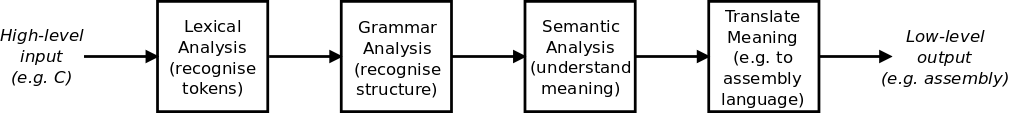
\includegraphics[width= 0.9\textwidth]{parsing_steps.png}
\end{figure}

\begin{itemize}
    \item Do \href{https://en.wikipedia.org/wiki/Lexical_analysis}{lexical analysis} to recognise the lexical elements. In several languages, {\color{red}=} is different to {\color{red}==}, so you can't just read a single {\color{red}=}. We call these lexical elements \textit{tokens}.
    \item \href{https://en.wikipedia.org/wiki/Parsing}{Parse} the input, i.e. recognise the syntax and structural elements of the input and ensure that they conform to the \textit{grammar} of the language. For example, your language might have this decision-making structure:
\end{itemize}

\begin{lstlisting}
    if (x < 23) {
        print("x is smaller than 23\n");
     }
\end{lstlisting}

but in another language you might write:

\begin{lstlisting}
    if (x < 23)
        print("x is smaller than 23\n");
\end{lstlisting}

This is also the place where the compiler cna detect syntax errors, like if the semicolon was missing on the end of first \textit{print} statement.

\begin{itemize}
    \item Do \href{https://en.wikipedia.org/wiki/Semantic_analysis_(compilers)}{semantic analysis} of the input, i.e. understand the meaning of the input. This is actually different from recognising the syntax and structure. For example, in English, a sentence might have the form '\textbf{<subject> <verb> <adjective> <object>}'.
\end{itemize}

\begin{lstlisting}
    David ate lovely bananas.
    Jennifer hates green tomatoes.
\end{lstlisting}

\begin{itemize}
    \item \href{https://en.wikipedia.org/wiki/Code_generation_(compiler)}{Translate} the meaning of the input into a different language. Here we convert the input, parts at a time, into a lower-level language.
\end{itemize}

\subsection{Resources}

There's a lot of comipler resources out on the Internet. Here are the ones I'll be looking at.

\section{Introducation}

\end{document}
